\documentclass{article}
\usepackage[utf8]{inputenc}
\usepackage{geometry}
\usepackage{graphicx}
\usepackage{amsmath}
\usepackage{amsfonts}
\usepackage{amsthm}
\usepackage{amssymb}
\usepackage[most]{tcolorbox}
\usepackage{array}
\usepackage{latexsym}
\usepackage{alltt}
\usepackage{hyperref}
\usepackage{color}
\usepackage{float}
\usepackage{pdfpages}
\usepackage{algpseudocode}
\usepackage{multicol}
\usepackage{multirow}
\usepackage{caption}
\usepackage{xparse}
\usepackage{setspace}
\usepackage{enumitem}
\usepackage{pdflscape}
\usepackage{parskip}

\geometry
{
  a4paper,
  left=15mm,
  right=15mm,
  top=15mm,
  bottom=15mm,
}

% parskip
\setlength{\parindent}{16pt}

% multicolumns
\setlength{\columnsep}{1.6\columnsep}
\setlength{\columnseprule}{0.2pt}

% mybox
\newtcolorbox{mybox}[3][]
{
  colframe = #2!25,
  colback  = #2!10,
  coltitle = #2!20!black,  
  title    = {#3},
  #1,
}

% New environments that use mybox
\newcounter{example}
\newenvironment{example}[1]{\begin{mybox}{green}{\refstepcounter{example}\textbf{Example~\theexample #1}}}{\end{mybox}}

\newenvironment{examplebreak}[1]{\begin{mybox}[breakable]{green}{\refstepcounter{example}\textbf{Example~\theexample #1}}}{\end{mybox}}

\newcounter{definition}
\newenvironment{definition}[1]{\refstepcounter{definition}\begin{mybox}{blue}{\textbf{Definition~\thedefinition #1}}}{\end{mybox}}

\newcounter{theorem}
\newenvironment{theorem}[1]{\begin{mybox}{red}{\refstepcounter{theorem}\textbf{Theorem~\thetheorem #1}}}{\end{mybox}}

\newenvironment{formula}[1]{\begin{mybox}{cyan}{\textbf{#1}}}{\end{mybox}}

% Changing maketitle
\makeatletter         
\renewcommand\maketitle{
{\raggedright % Note the extra {
\begin{center}
{\Large \bfseries \@title}\\[2ex] 
{\large \@author \ - \@date}\\[2ex]
\end{center}}} % Note the extra }
\makeatother

% \onehalfspacing % adjust spacing

% macros
\newcommand{\prob}[1]{\textbf{\textit{P}}\{#1\}}
\NewDocumentCommand{\dsum}{%
    e{^_}
}{%
  {% 
    \displaystyle\sum
    \IfValueT{#1}{^{#1}}
    \IfValueT{#2}{_{#2}}
  }
}%

% maketitle variables
\title{CENG 222 - Chapter 8: Introduction to Statistics}
\author{Burak Metehan Tunçel}
\date{April 2022}

\begin{document}

\maketitle

\begin{multicols}{2}
  We learned analyzing problems and systems involving uncertainty, to find \textit{probabilities, expectations}, and \textit{other characteristics} for a variety of situations, and to produce forecasts that may lead to important decisions.

  What was given to us in all these problems? Ultimately, \textit{we needed to know the distribution and its parameters}, in order to compute probabilities or at least to estimate them by means of Monte Carlo. Often the distribution may not be given, and we learned how to fit the suitable model, say, Binomial, Exponential, or Poisson, given the type of variables we deal with. In any case, parameters of the fitted distribution had to be reported to us explicitly, or they had to follow directly from the problem.

  This, however, is rarely the case in practice. Only sometimes the situation may be under our control, where, for example, produced items have predetermined specifications, and therefore, one knows parameters of their distribution.

  Much more often \textit{parameters are not known}. To apply the knowledge we learned, \textit{we need to collect data}. A properly collected sample of data can provide rather sufficient information about parameters of the observed system. We will learn how to use this sample
  \begin{itemize}
    \item to visualize data, understand the patterns, and make quick statements about the system's behavior;
    \item to characterize this behavior in simple terms and quantities;
    \item to estimate the distribution parameters;
    \item to assess reliability of our estimates;
    \item to test statements about parameters and the entire system;
    \item to understand relations among variables;
    \item to fit suitable models and use them to make forecasts
  \end{itemize}
\end{multicols}

\section{Population and Sample, Parameters and Statistics}

Data collection is a crucially important step in Statistics. We use the collected and observed sample to make statements about a much larger set - the population.

\begin{definition}{}
  A \textbf{population} consists of all units of interest. Any numerical characteristic of a population is a \textbf{parameter}. A \textbf{sample} consists of observed units collected from the population. It is used to make statements about the population. Any function of a sample is called \textbf{statistic}.
\end{definition}

In real problems, we would like to make statements about the population. To compute probabilities, expectations, and make optimal decisions under uncertainty, we need to know the population \textit{parameters}. However, the only way to know these parameters is to measure the entire population, i.e., to conduct a census.

Instead of a census, we may \textit{collect data in a form of a random sample from a population} (Figure 1). This is our data. We can measure them, perform calculations, and estimate the unknown parameters of the population up to a certain measurable degree of accuracy.

\begin{figure}[ht]
  \centering
  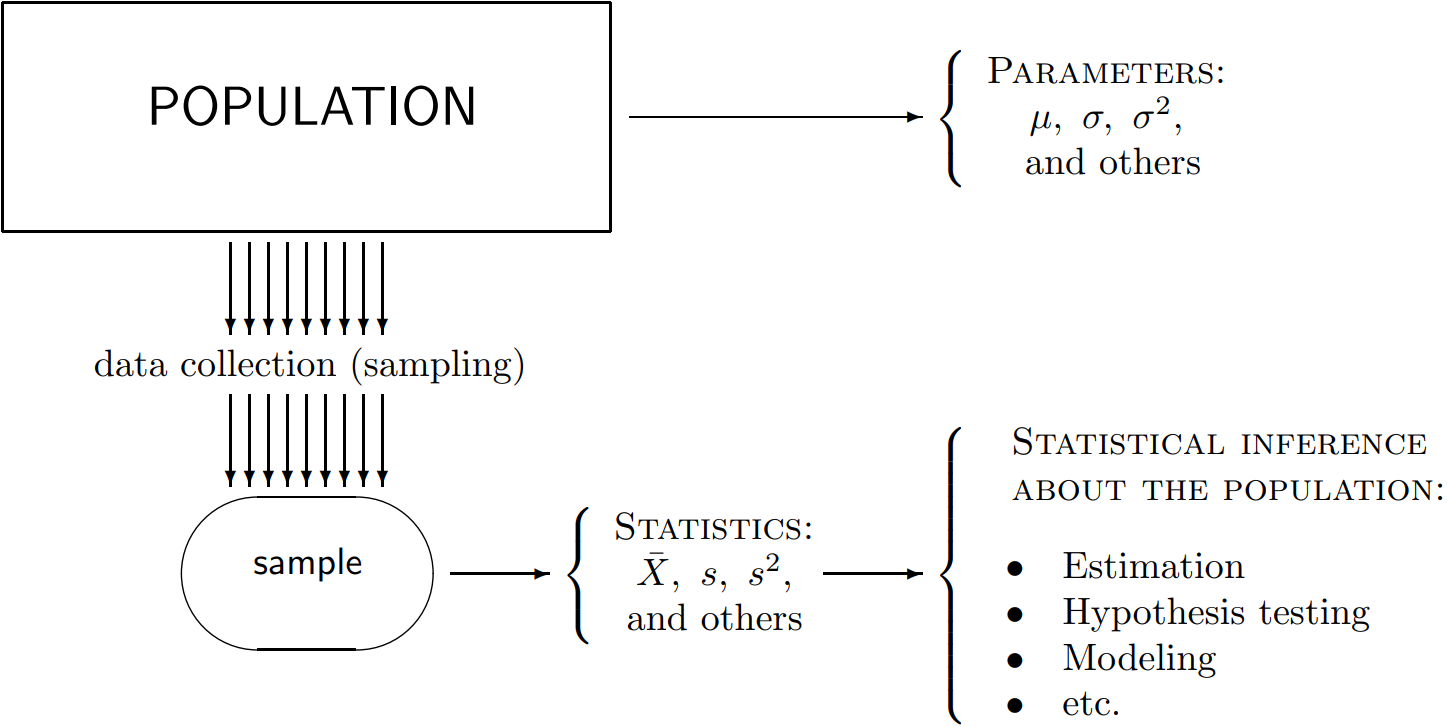
\includegraphics[width=.7\textwidth]{img/fig8-1.png}
  \caption{\textit{Population parameters and sample statistics.}}
\end{figure}

A sample may sometimes give a rather misleading information about the population although this happens with a low probability. \textit{Sampling errors cannot be excluded}.

\subsection{Sampling and Non-sampling Errors}

Sampling and non-sampling errors refer to any discrepancy between a collected sample and a whole population.
\begin{itemize}
  \item \textbf{Sampling errors} are caused by the mere fact that \textit{only a sample, a portion of a population, is observed}. For most of reasonable statistical procedures, \textit{sampling errors decrease (and converge to zero) as the sample size increases}.
  \item \textbf{Non-sampling errors} are caused by \textit{inappropriate sampling schemes or wrong statistical techniques}. Often no wise statistical techniques can rescue a poorly collected sample of data.
\end{itemize}

\noindent \textit{\textbf{Note:} Check the examples 8.1-8.5 in the textbook.}

We will focus on \textit{simple random sampling}, which is one way to avoid non-sampling errors.

\begin{definition}{}
  \textbf{Simple random sampling} is a sampling design where units are collected from the entire population independently of each other, all being equally likely to be sampled.
\end{definition}

Observations collected by means of a simple random sampling design are \textbf{iid} (\textit{independent, identically distributed}) random variables.

\begin{example}{}
  To evaluate its customers' satisfaction, a bank makes a list of all the accounts. A Monte Carlo method is used to choose a random number between 1 and $N$, where $N$ is the total number of bank accounts. Say, we generate a Uniform$(0,N)$ variable $X$ and sample an account number $\left\lceil X \right\rceil$ from the list. Similarly, we choose the second account, uniformly distributed among the remaining $N - 1$ accounts, etc., until we get a sample of the desired size $n$. This is a simple random sample.
\end{example}


\end{document}
